\documentclass[a4paper]{article}

\usepackage[english]{babel}
\usepackage[utf8]{inputenc}
\usepackage{amsmath}
\usepackage{graphicx}

\title{Project Report\\ Flow-Based Image Abstraction}

\author{
	Mayank Meghwanshi\\ \texttt{110050012} 
    \and 
    Vivek Atulkar\\ \texttt{110050039}
    }

\date{\today}

\begin{document}
\maketitle


\section{Problem Statement}

We implemented image toonificaton technique based on the paper Flow-Based Image Abstraction\cite{10.1109/TVCG.2008.81}. The approach is based on shape/color filtering guided by edge tangent field which improves abstraction performance in terms of feature enhancement and stylizations. 
\\
We implemented following two subproblem of image abstraction
\begin{enumerate}
\item \textbf{Line Extraction} - Using Flow-based Difference of Gaussian (FDoG).
\item \textbf{Region Smoothing} - Using Flow-based Bilateral Filter (FBL).
\end{enumerate}

\section{Algorithms Implemented}

\subsection{Flow Construction - Edge Tangent Flow}

Edge Tangent Flow(ETF) is smooth, feature preserving edge flow field which is used as guiding map for further steps of the filter. \textit{Edge tangent} is defined as vector perpendicular to image gradient, and it represents tangent of local edge flow. 
\\
\textbf{Input} - Gray-scaled image, Kernel radius($\mu$), Number of Iterations\\
\textbf{Output} - Tangent direction vectors at each pixel\\
\textbf{Steps}
\begin{enumerate}
\item Initialize tangent flow using initial gradient map calculate using sobel operators.
\item Now iteratively update the tangent flow using ETF construction filter described in the paper. \\ETF construction filter is combination of \textit{spatial weight function}, \textit{magnitude weight function} and \textit{direction weight function}
\item Figure \ref{fig:ETF} shows 3 iterations of ETF filter. 
\begin{figure}
\centering
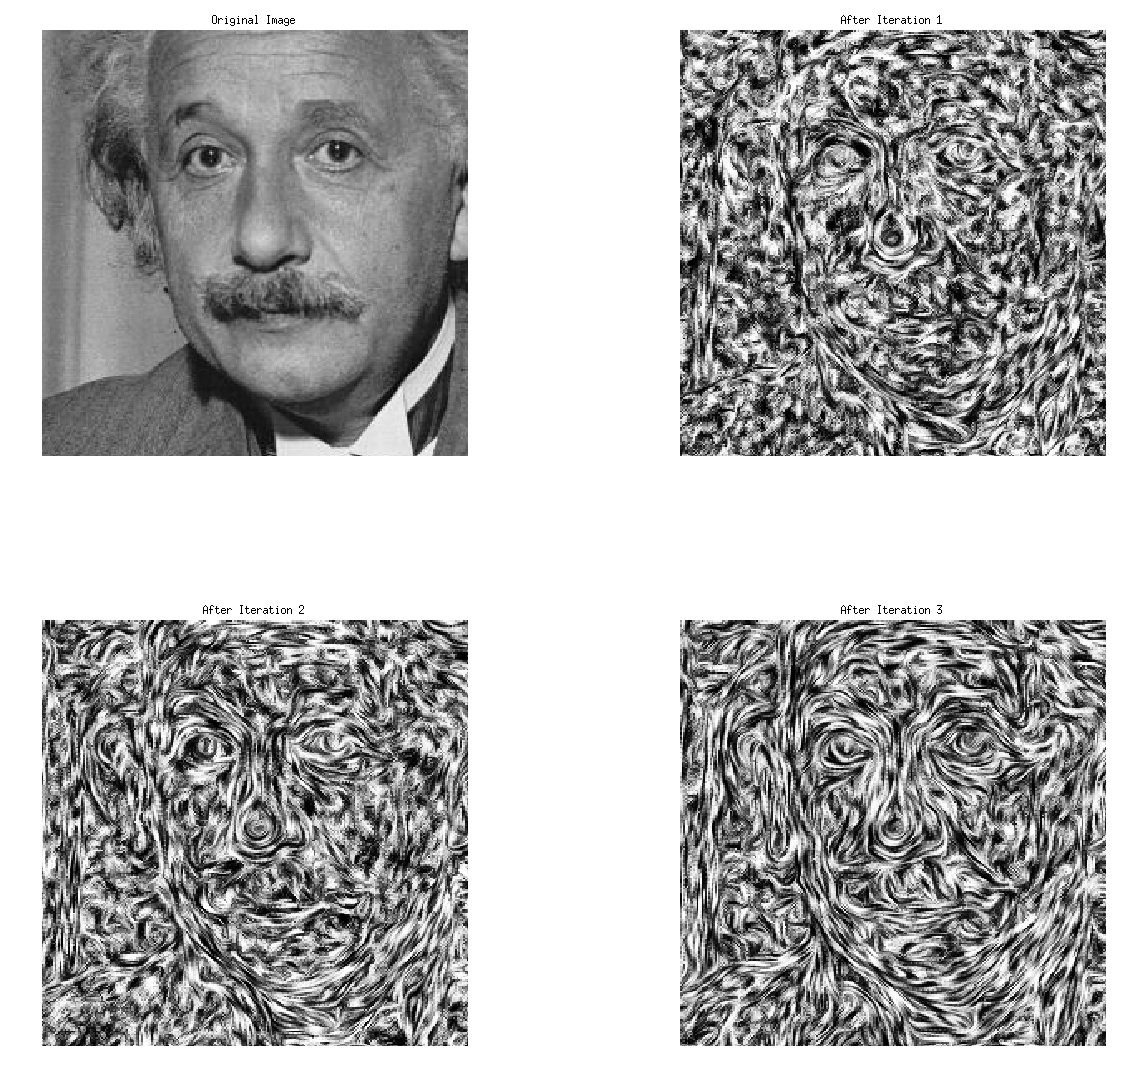
\includegraphics[width=1\textwidth]{ETF.png}
\caption{\label{fig:ETF}Edge tangent flow. It grows progressively smoother with each iteration.}
\end{figure}
\end{enumerate}



\subsection{Line Extraction - Flow-based Difference of Gaussian Filter}

ETF gives us the local tangent direction of the image. In FDoG filter we use this information and apply Difference of Gaussian filter along the perpendicular direction which is more likely to give highest contrast. Then we move along the flow to collect enough information to find genuine edges.
\\
\textbf{Input} - Gray-scaled image, Tangent directions, $\sigma_m$, $\sigma_c$, $\rho$, $\tau$, Number of iterations
\begin{itemize}
\item $\sigma_m$ - Represents Gaussian along the tangential direction controls degree of line coherence.
\item $\sigma_c$ - Represents one of the Gaussian used in DoG filter determines width of resulting line.
\item $\rho$ - Controls the noise detected.
\item $\tau$ - Serves as the threshold for binarization of the image.
\end{itemize}
\textbf{Output} - Binary Edge Image\\
\textbf{Steps}
\begin{enumerate}
\item First we take $2\beta$ points along the perpendicular direction of tangent and apply DoG filter on it, do this for all pixels.
\item Then take $2\alpha$ points along the direction of tangent and apply Gaussian filter on it, do this for all pixels.
\item Use thresholding to generate binarized image.
\item To apply FDoG iteratively first merge edge image to original image and then do above steps again. Figure \ref{fig:fdog} shows 3 iterations.
\begin{figure}
\centering
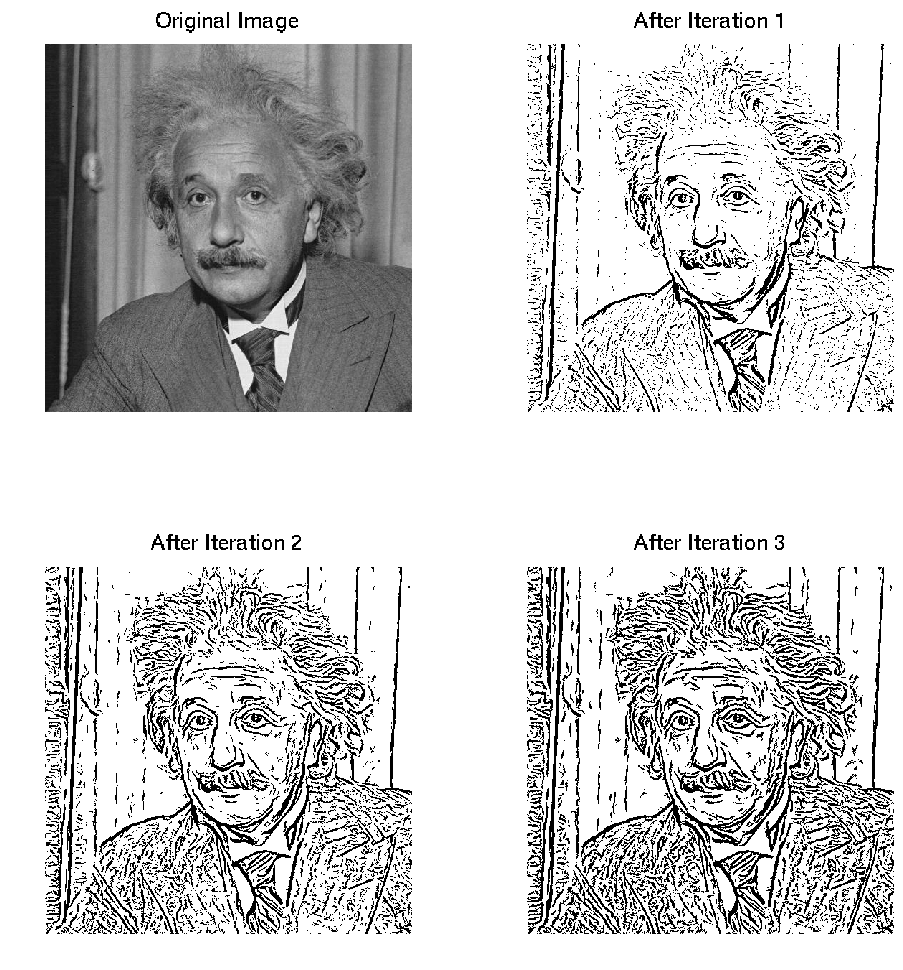
\includegraphics[width=1\textwidth]{fdog.png}
\caption{\label{fig:fdog}Flow-based DoG. Progressively improves edge coherence}
\end{figure}
\end{enumerate}


\subsection{Region Smoothing - Flow-Based Bilateral Filter}
We use two filters in FBL, first along the tangent direction and next along the gradient direction(perpendicular to tangent).  First operates in edge directions and cleans out shape boundaries and the other one acts perpendicular and smooths out region interiors. 
\\
\textbf{Input} - Original Image, Tangent directions, $\sigma_e$, $r_e$, $\sigma_g$, $r_g$
\begin{itemize}
\item $\sigma_e$ - Spatial weight function(Gaussian) along the edge direction
\item $r_e$ - Similarity weight function along the edge direction on difference of color
\item $\sigma_g$ - Spatial weight function(Gaussian) along the gradient direction
\item $r_g$ - Similarity weight function along the gradient direction on difference of color
\end{itemize}
\textbf{Output} - Smoothened Image\\
\textbf{Steps}
\begin{enumerate}
\item First we take $2\alpha$ points along the edge direction and apply linear bilateral filter on it.
\item Then we take $2\beta$ points along the gradient direction and apply linear bilateral filter on it.
\item Apply the mask iteratively. Figure \ref{fig:fbl} shows 2 iterations of FBL.
\begin{figure}
\centering
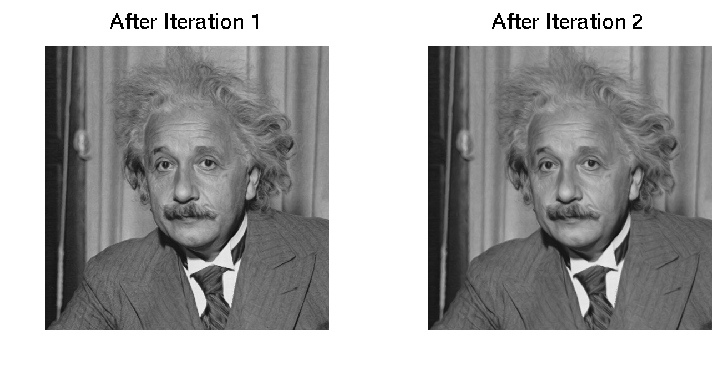
\includegraphics[width=1\textwidth]{fbl.png}
\caption{\label{fig:fbl}Flow-based Bilateral Filter.}
\end{figure}
\end{enumerate}

\subsection{Region Flattening - Luminance Quantization}
We quantize the filtered image by uniform-sized-bin luminance quantization. 
For gray-scale image we quantize directly according to the intensity value. For RGB image first we convert it into Cie-LAB color-map and apply the quantization on luminance part of the image. Then we convert back to RGB image. Figure \ref{fig:quant} shows quantized image.
\begin{figure}
\centering
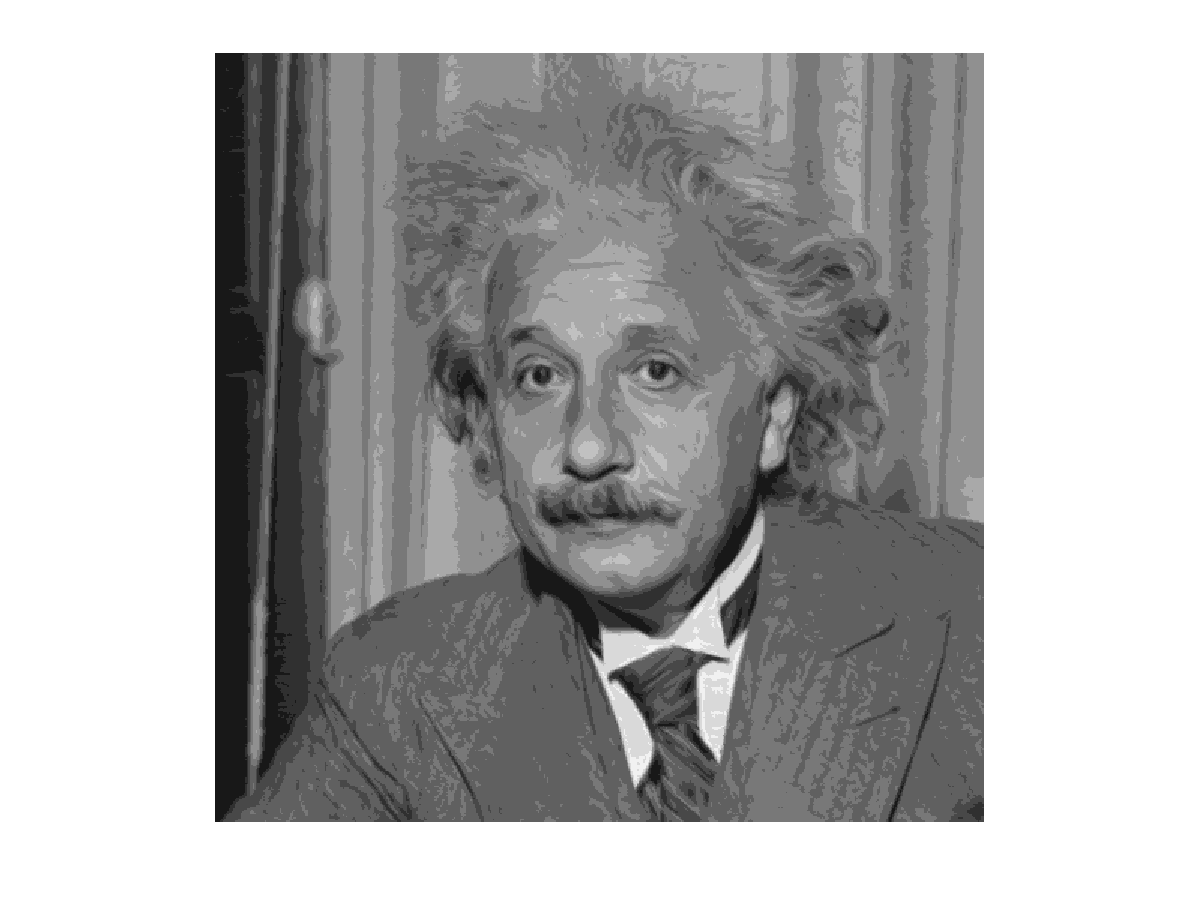
\includegraphics[width=1\textwidth]{quant.png}
\caption{\label{fig:quant}Quantized Image.}
\end{figure}

\begin{figure}
\centering
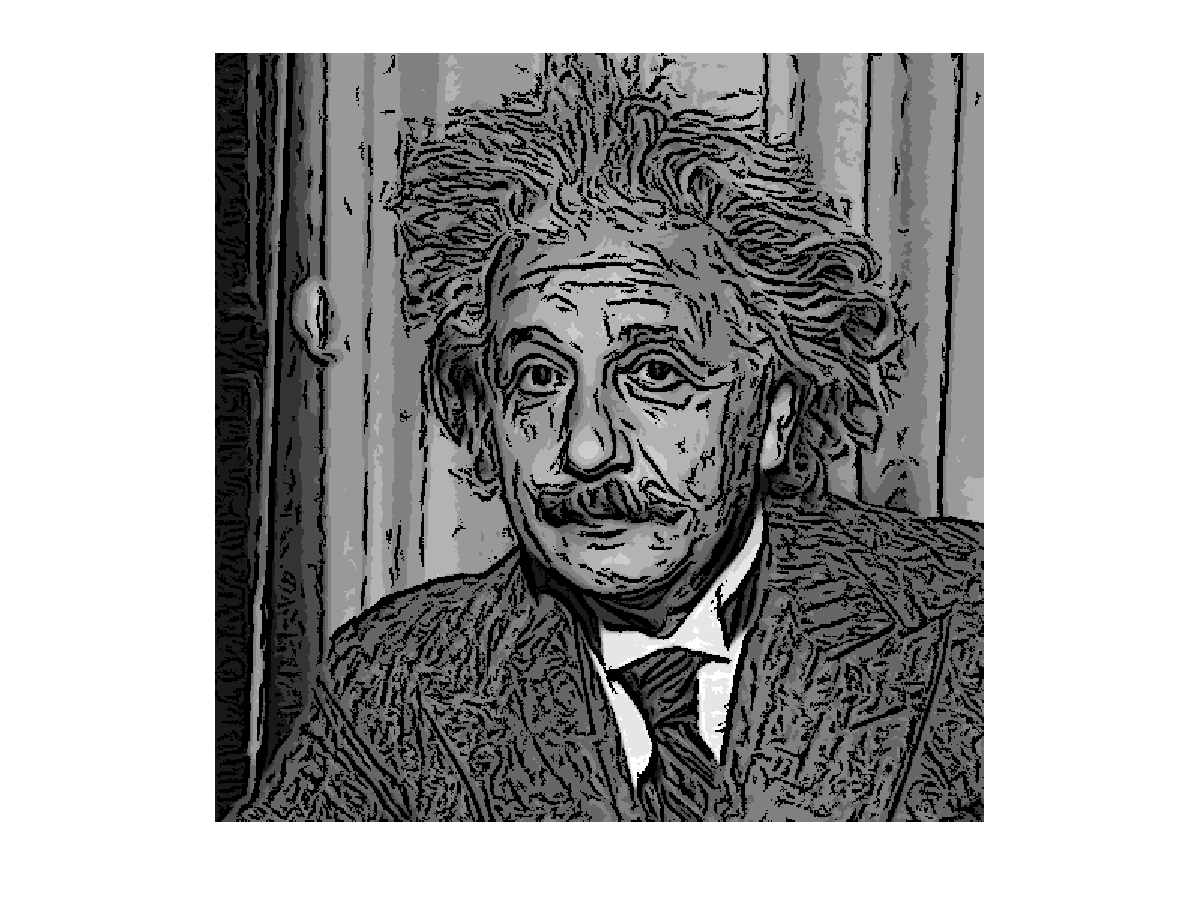
\includegraphics[width=1\textwidth]{final.png}
\caption{\label{fig:final}Final Merged Image.}
\end{figure}

\begin{figure}
\centering
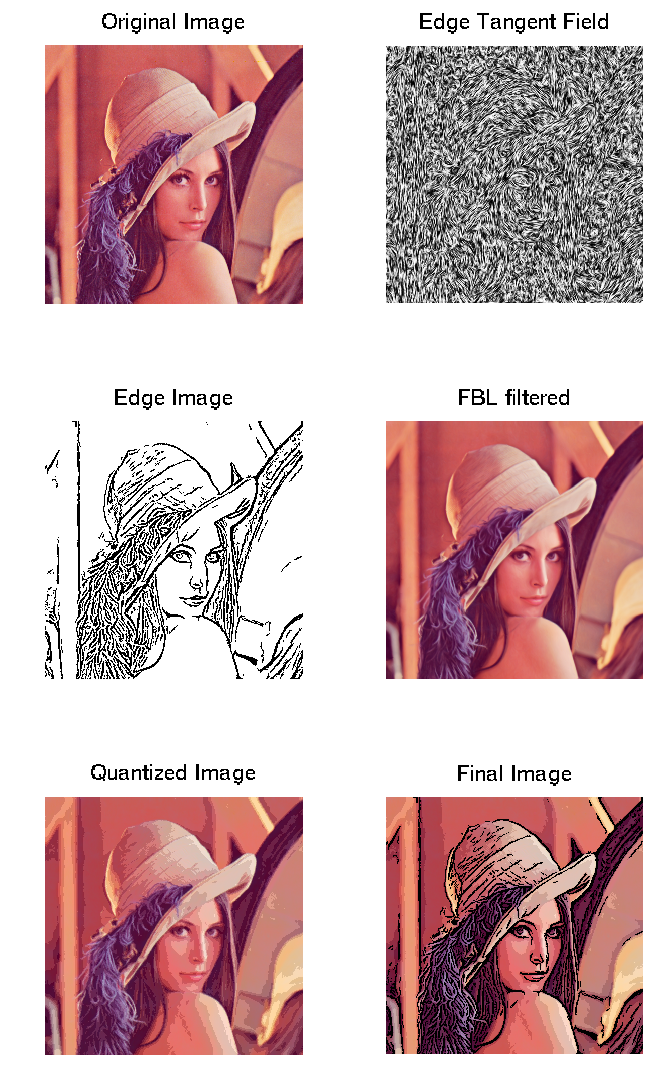
\includegraphics[width=1\textwidth]{lenna_final.png}
\caption{Lenna Image}
\end{figure}

\begin{figure}
\centering
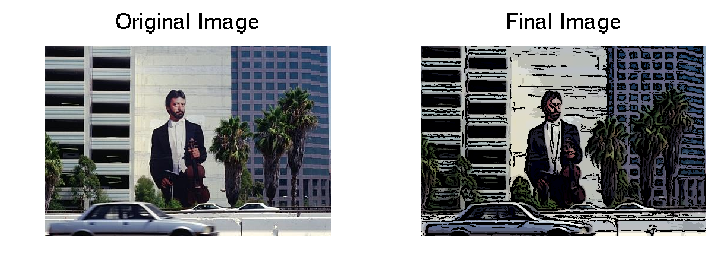
\includegraphics[width=1\textwidth]{119082_final.png}
\caption{Sample Image 1}
\end{figure}

\begin{figure}
\centering
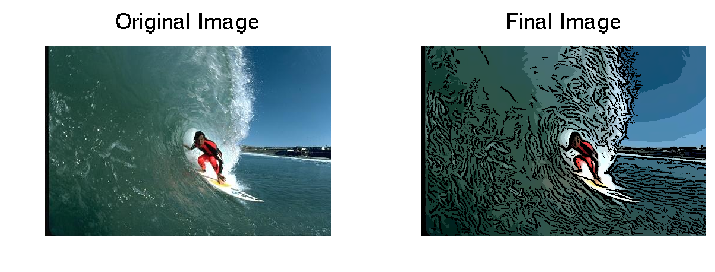
\includegraphics[width=1\textwidth]{300091_final.png}
\caption{Sample Image 2}
\end{figure}
\begin{figure}
\centering
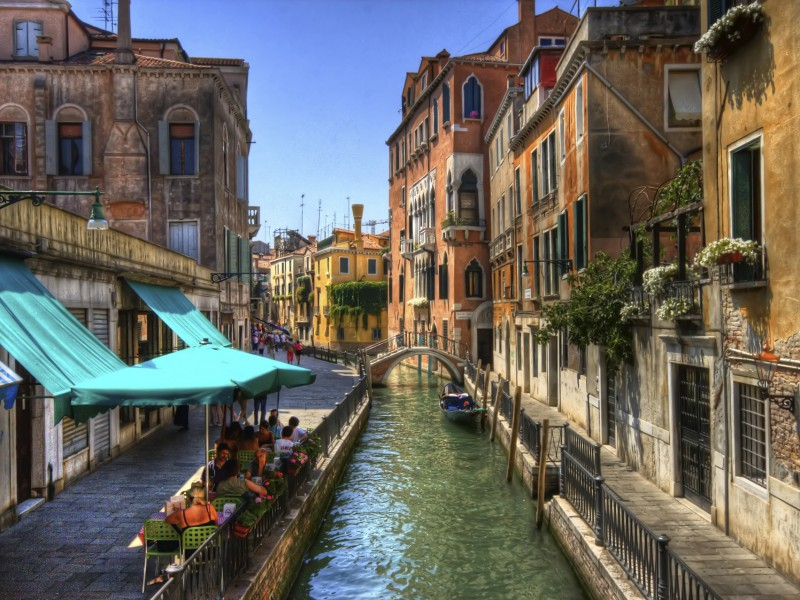
\includegraphics[width=1\textwidth]{narrow_canal.jpg}
\caption{Sample Image 3 - Original}
\end{figure}
\begin{figure}
\centering
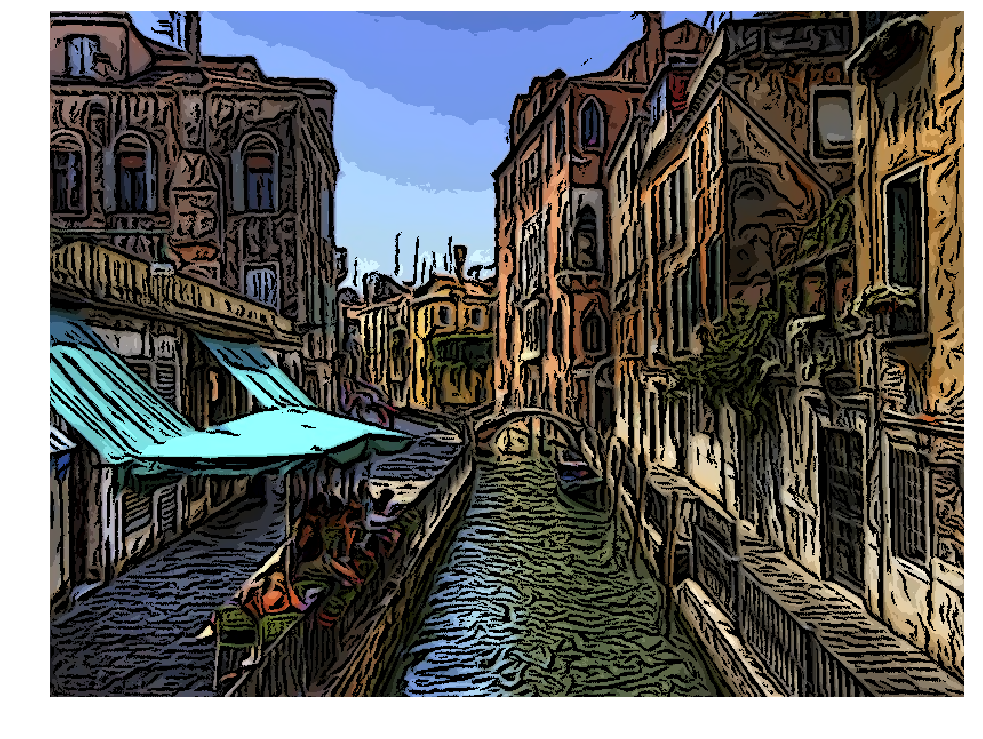
\includegraphics[width=1\textwidth]{narrow_canal_final.png}
\caption{Sample Image 3 - Final}
\end{figure}


\newpage
\subsection{Limitations}
\begin{itemize}
\item This approach depends completely upon accuracy of underlying vector field ETF, if that is not properly represent local features then it is not possible to abstract that detail. 
\item ETF is also not capable of preserving finer texture of the image, which requires it to have small kernel radius.
\item This approach have a lot of parameters at each step, for each image the best parameters to set might be different and is subjective in nature.
\item Our implementation of FDoG filter does not give as good results as shown in the paper, and shows too many unnecessary edges.
\end{itemize}

\subsection{Advantages}
\begin{itemize}
\item This algorithm uses two linear bilateral filters instead of single 2-D bilateral filter, which speeds it up relative to traditional bilateral filter.
\item This algorithm give thicker and more coherent edges, which are perceptually more meaningful then given by other edge detection algorithms.
\item ETF filters enables it to smoothen along the edge and perpendicular to edge separately. Which protects edges and smooths out interior.
\end{itemize}

\subsection{Work Division}
Most of the time we worked together while working on the project and each of us have equal contribution to the project.


\bibliographystyle{plain}
\bibliography{bibliography.bib}

\end{document}